\documentclass[11pt]{article}

\usepackage[ngerman]{babel}
\usepackage[T1]{fontenc}
\usepackage{fontspec}
\setmainfont{Arial}
\usepackage{graphicx}
\usepackage{makeidx}
\usepackage[hidelinks]{hyperref}
\usepackage[a4paper, head=50pt]{geometry}
\usepackage{fontawesome}
\usepackage{xcolor}
\usepackage{xifthen}
\usepackage{scrlayer-scrpage}
\usepackage[toc=false]{glossaries-extra}
\usepackage[normalem]{ulem}
\usepackage{graphicx}
\graphicspath{ {./images/} }
\usepackage{multirow}
\usepackage{setspace}
\usepackage{pdfpages}
\usepackage{lscape}

\usepackage[
backend=biber,
style=alphabetic,
sorting=ynt
]{biblatex}

\title{Travel-Assistant}
\author{Ricardo Hoffmann}
\date{17. April 2024}

\definecolor{link}{HTML}{0000EE}
\definecolor{todo}{HTML}{FF0000}
\newcommand{\todo}{\textcolor{todo}{// TODO!}}

\newcommand{\link}{\faLink}
\newcommand{\extlink}{\faExternalLink}

\newcommand{\ext}[2][]{\textcolor{link}{\href{#2}{\ifthenelse{\equal{#1}{}}{#2}{#1}\,\faExternalLink}}}
\newcommand{\sct}[2]{\textcolor{link}{\hyperref[#1]{#2\,\faLink}}}
\newcommand{\gl}[1]{\dotuline{\gls{#1}}}
\newcommand{\glp}[1]{\dotuline{\glspl{#1}}}

\newcommand{\qt}[1]{\glqq#1\grqq}

\setstretch{1.3}
\setlength{\parindent}{0cm}
\newglossaryentry{RA}{
  name={RA},
  description={Reisekostenabrechnung},
  first={Reisekostenabrechnung (\glsentrytext{RA})},
  plural={RAs},
  descriptionplural={Reisekostenabrechnungen},
  firstplural={Reisekostenabrechnungen (\glsentryplural{RA})}
}
\newglossaryentry{MED}{
  name={MED},
  description={Microsoft Excel Datei},
  first={Microsoft Excel Datei (MED)},
  plural={MEDs},
  descriptionplural={Microsoft Excel Dateien},
  firstplural={Microsoft Excel Datei (\glsentryplural{MED})}
}
\newglossaryentry{IDP}{
  name={IdP},
  description={Identity Provider},
  first={Identity Provider (\glsentrytext{IDP})}
}
\newglossaryentry{MA}{
  name={MA},
  description={Mitarbeiter},
  first={Mitarbeiter (\glsentrytext{MA})}
}
\newglossaryentry{GF}{
  name={GF},
  description={Geschäftsführung},
  first={Geschäftsführung (\glsentrytext{GF})}
}
\newglossaryentry{HTTP}{
  name={HTTP},
  description={\emph{\textbf{H}yper\textbf{t}ext \textbf{T}ransfer \textbf{P}rotocol}}
}
\newglossaryentry{API}{
  name={API},
  description={\emph{\textbf{A}pplication \textbf{P}rogramming \textbf{I}nterface}}
}
\newglossaryentry{mongoose}{
  name={Mongoose},
  description={\gl{ODM}-Library zur Verbindung mit \gl{MongoDB}, \ext{https://mongoosejs.com}}
}
\newglossaryentry{SPA}{
  name={SPA},
  description={\emph{\textbf{S}ingle \textbf{P}age \textbf{A}pplication}}
}
\newglossaryentry{MongoDB}{
  name={MongoDB},
  description={Dokumentenbasiertes NoSQL-Datenbanksystem, \ext{https://www.mongodb.com}}
}
\newglossaryentry{ODM}{
  name={ODM},
  description={\emph{\textbf{O}bject \textbf{D}ata \textbf{M}odeling}}
}
\newglossaryentry{JS}{
  name={JavaScript},
  description={Skriptsprache, die eine der Haupttechnologien des WWW ist}
}
\newglossaryentry{React}{
  name={React},
  description={Open Source Single Page Application Framework. Umfasst vergleichsweise geringen Funktionsumfang out-of-the-box, ist im Umkehrschluss aber wesentlich flexibler und zum Beispiel im Web und Nativ anwendbar}
}
\newglossaryentry{HTML}{
  name={HTML},
  description={\emph{\textbf{H}yper\textbf{t}ext \textbf{M}arkup \textbf{L}anguage}, \gl{XML}-basierte Beschreibungsnotation für Webumgebungen}
}
\newglossaryentry{XML}{
  name={XML},
  description={\emph{e\textbf{X}tensible \textbf{M}arkup \textbf{L}anguage}}
}
\newglossaryentry{MSC}{
  name={MSC},
  description={\emph{\textbf{M}odel, \textbf{S}ervice, \textbf{C}ontroller}, Architektur zur Gestaltung von Applikationen}
}
\newglossaryentry{GUI}{
  name={GUI},
  description={\emph{\textbf{G}raphical, \textbf{U}ser, \textbf{I}nterface}, Grafische Benutzeroberfläche}
}
\newglossaryentry{nodejs}{
  name={Node.js},
  description={\gl{JS}-Laufzeitumgebung, \url{https://nodejs.com}}
}
\newglossaryentry{vite}{
  name={vite},
  description={Buildtool für diverse \gl{SPA}-Frameworks, \ext{https://vitejs.dev}}
}
\newglossaryentry{cookie}{
  name={Cookie},
  description={kleine Textdaten, die vom Browser gespeichert und bei \gl{HTTP}-Requests mitgesendet werden}
}
\newglossaryentry{jwt}{
  name={JWT},
  description={\emph{\gl{json} \textbf{W}eb \textbf{T}oken}, \ext{https://jwt.io/introduction}}
}
\newglossaryentry{json}{
  name={JSON},
  description={\emph{\gl{JS} \textbf{O}bject \textbf{N}otation}, Textbasiertes Datenformat zum Datenaustausch zwischen mehreren Anwendungen}
}
\newglossaryentry{CRUD}{
  name={CRUD},
  description={\emph{\textbf{C}reate, \textbf{R}ead, \textbf{U}pdate, \textbf{D}elete}}
}
\newglossaryentry{git}{
  name={Git},
  description={Versionsverwaltungssystem, \ext{https://git-scm.com}}
}
\newglossaryentry{vscode}{
  name={Visual Studio Code},
  description={Entwicklungsumgebung/Texteditor, \url{https://code.visualstudio.com}}
}
\newglossaryentry{miro}{
  name={miro},
  description={Online-Kollaborationsplattform für u.a. Diagramme, Mindmaps und Unterschiedliche Boards, \url{https://miro.com/de/}}
}
\newglossaryentry{MERN}{
  name={MERN},
  description={Ein Technologie-Stack, welcher aus den Komponenten: \gl{MongoDB}, \gl{express}, \gl{React} und Node.js. besteht }
}
\newglossaryentry{express}{
  name={Express},
  description={ein serverseitiges Webframework für die JavaScript-basierte Plattform Node.js, \url{https://expressjs.com} }
}
\newglossaryentry{JSdoc}{
  name={JSdoc},
  description={eine Auszeichnungssprache, die zum Annotieren von JavaScript-Quellcodedateien verwendet wird, \url{https://jsdoc.app/} }
}
\newglossaryentry{cors}{
  name={CORS},
  description={\textbf{C}ross-\textbf{O}rigin \textbf{R}esource \textbf{S}haring }
}
\newglossaryentry{promise}{
  name={Promise},
  description={\gl{JS}-\gl{API} zum Abhandeln von asynchron ablaufenden Prozessen. engl. Promise: Versprechen, es wird \texttt{await}-ed, dass die Promise eingelöst wird und man so die Daten erhält}
}
\newglossaryentry{css}{
  name={CSS},
  description={\emph{\textbf{C}ascading \textbf{S}tyle\textbf{s}heets}}
}
\newglossaryentry{jest}{
  name={jest},
  description={ein \gl{JS} Testing Framework}
}
\glsaddall
\makenoidxglossaries

\glsaddall
\makenoidxglossaries

\begin{document}

\makeatletter
\let\doctitle\@title
\let\docauthor\@author
\let\docdate\@date
\makeatother

\pagenumbering{gobble}

\begin{titlepage}
    \begin{center}
        \vspace{0.5cm}
        
        
\includegraphics[width=0.6\textwidth]{IHK-Logo-Ostwestfalen.png}
        
        \vspace{0.5cm}
        
        Abschlussprüfung Sommer 2024\\
        Fachinformatiker für Anwendungsentwicklung\\
        \Large
        Dokumentation zur betrieblichen Projektarbeit
        
        \vspace{0.5cm}
        
        \LARGE
        \textbf{\doctitle}
        
        \Large
        \vspace{0.5cm}
        Digitalisierung von Erstellung, Verwaltung \& Validierung der Reisekostenabrechnungen mithilfe einer Single-Page-Application
        
        \vspace{0.5cm}
        \textbf{\docdate}
        
        \vspace{1.5cm}
        
        \large
        \textbf{\docauthor}\\
        Elpke 19a\\
        33605 Bielefeld
            
        \vfill
        
        \begin{minipage}{0.3\textwidth}
        \centering
            
\includegraphics[width=0.5\textwidth]{DTS}
        \end{minipage}
        \begin{minipage}{0.45\textwidth}
        \centering
            \textbf{Ausbildungsbetrieb:}\\
            DTS Systeme GmbH\\
            Schrewestraße 2\\
            32051 Herford
        \end{minipage}
            
    \end{center}
\end{titlepage}

\tableofcontents
\pagebreak
\vfill
Legende:
\begin{enumerate}
  \item \textcolor{link}{Links innerhalb des Dokuments \link}
  \item \textcolor{link}{Links zu externen Internetseiten \extlink}
  \item \dotuline{Links zu Glossareinträgen} 
\end{enumerate}

\pagenumbering{arabic}
\setcounter{page}{4}

\setlength{\parskip}{0.2cm}

\pagestyle{scrheadings}

\ihead{\doctitle\\
\headmark}
\ohead{
\includegraphics[width=1.5cm]{DTS}}
\ifoot{\docauthor}
\ofoot{\pagemark}
\automark{section}

\section{Einführung und Definitionsphase}
\label{sec:Einführung-Definitionsphase}
\input{sections/einführung-definitionsphase}

\section{Projektplanung}
\label{sec:Projektplanung}
\subsection{Projektphasen und Zeitplanung}

Wie von der IHK Ostwestfalen zu Bielefeld vorgegeben, stehen für die Durchführung dieses Projektes 80 Stunden zur Verfügung. Eine Übersicht über die ursprüngliche Schätzung der Arbeitspakete (und die tatsächlich benötigte Zeit) kann dem Soll/Ist Vergleich entnommen werden.

\subsection{Ressourcenplanung}

Eine Übersicht über die Ressourcen erstellt, die voraussichtlich während der Projektlaufzeit benötigt werden. Diese wurde während der Projektlaufzeit laufend aktualisiert, so dass auch spontan hinzukommende Ressourcen abgebildet sind. Die Ressourcenplanung ist im Anhang unter Verwendete Ressourcen zu finden\todo. Bei der Auswahl der Software wurde darauf geachtet, dass bereits Kenntnisse oder Erfahrungen mit der jeweiligen Software vorhanden waren, um einen möglichen Zeitverlust durch Einarbeitung möglichst gering zu halten. Darüber hinaus wurden die jeweiligen Lizenz- und Nutzungsbedingungen der verschiedenen Lösungen berücksichtigt.


\section{Analysephase}
\label{sec:Analysephase}
\subsection{Ist-Analyse}

Wie bereits unter \sct{sec:Einführung-Definitionsphase:Ausgangssituation}{Ausgangssituation} beschrieben, wird derzeit eine veraltete und unübersichtliche / fehleranfällige \gl{MED} zur Erstellung der \gl{RA} verwendet. 

\subsubsection{Reisekostenabrechnungsprozess}
\label{sec:Analysephase:Reisekostenabrechnungsprozess}

Der \gl{MA} im Außendienst füllt die \gl{RA} aus und legt sie seinem Vorgesetzten (und ggf. der \gl{GF}) vor, welche prüfen, ob die Dienstreise(n) genehmigt wurde(n). Ist dies der Fall, wird diese an die Payroll Accounting Abteilung weitergeleitet und dort auf Manipulationen, wie z.B. falsche Pauschalbeträge (die als Berechnungsgrundlage dienen), überprüft. Weist die \gl{RA} keine Manipulationen vor, kann sie an die Accountig Abteilung weitergeleitet werden, die die Berechnungen und die Übereinstimmung der Belege mit den eingetragenen Kosten überprüft. Ist die \gl{RA} in Ordnung, kann eine entsprechende Auszahlung veranlasst werden. Sollte jedoch in einem der oben genannten Fälle etwa mit der \gl{RA} nicht in Ordnung sein, muss diese vom Mitarbeiter bearbeitet werden oder wird schlichtweg abgelehnt.

Eine grobe Darstellung des aktuellen Prozesses der Reisekostenabrechnung ist in visueller Form im Anhang unter \sct{sec:Anhang:ProzessAlt}{Prozess Alt} zu finden.

\subsubsection{Herausforderungen}

Wie in der \sct{sec:Einführung-Definitionsphase:Ausgangssituation}{Ausgangssituation} beschrieben, ist diese \gl{MED} komplex, was zu Fehlern führt. Z.B. dass Bedingungen falsch verstanden werden und dementsprechend eingetragen werden, obwohl sie nicht eingetragen werden sollten. Grundsätzlich kann es aufgrund der Art der \gl{MED} zu Manipulationen der Berechnungslogik oder der Pauschalen kommen. Zudem kommt es häufig vor, dass notwendige Belege nicht beigefügt werden oder die angegebenen Kosten nicht validiert werden können. Diese Herausforderungen erschweren den Einsatz in den Abteilungen, in welchen diese verwendet wird.

\subsection{Soll-Zustand}

Die \gl{MED} soll durch eine moderne \gl{SPA} ersetzt werden. Diese  \gl{SPA} soll die Möglichkeit bieten, eine \gl{RA} digital zu erstellen, zu bearbeiten, freizugeben und zu prüfen. Ein regelbasierter Chatbot soll dem \gl{MA} zu der Dienstreise Fragen stellen und die Antworten im Hintergrund verarbeiten. Im Anhang unter \sct{sec:Anhang:Lastenheft}{Lastenheft} können nähere Details zum Soll-Zustand/Anforderungen entnommen werden.


\subsection{Wirtschaftlichkeit}
Da diese Softwarelösung die veraltete \gl{MED} ablösen soll, spielt die Wirtschaftlichkeit eine untergeordnete Rolle. Dennoch können monatliche Einsparungen erzielt werden, die sich anhand folgender Annahmen/Durchschnittswerten ergeben.

Von folgenden Personalkosten wird ausgegangen:
\begin{itemize}
\item Auszubildender/Autor: 7€/h
\item \gl{MA} im Außendienst: 25€/h
\item Junior Software Developer: 27€/h
\item Accounting Abteilung/ Payroll Accounting/ Betreuerin: 30€/h
\item Vorgesetzter: 45€/h
\item \gl{GF}: 100€/h
\end{itemize}

Folgende Annahmen gelten universell:
\begin{itemize}
\item 20 \glp{RA} werden im Monat eingereicht
\item Genehmigung des Vorgesetzten - 1 Vorgesetzter à 5 Minuten
\item Genehmigung der \gl{GF} - 1 \gl{GF} einmal im Monat à 5 Minuten
\item 10\% der Ersteller wenden sich mit Fragen direkt an die Account Abteilung - 1 \gl{MA} Accounting, 1 \gl{MA} im Außendienst à 10 Minuten
\end{itemize}

Folgende Annahmen gelten für den Prozess rund um die \gl{RA} mit der bestehenden \gl{MED}:
\begin{itemize}
\item \gl{RA} erstellen - 1 \gl{MA} im Außendienst à 15 Minutent
\item Jeden 2. Monat Einführung eines \gl{MA} - 2 \gl{MA} im Außendienst à 1 Stunde
\item 20\% der Ersteller bitten Kollegen um Hilfe - 2 \gl{MA} im Außendienst à 15 Minuten
\item 90\% der \glp{RA} wird über die Hauspost geliefert - 1 Auszubildender à 10 Minuten
\item 10\% der \glp{RA} persönlich eingereicht – 1 \gl{MA} im Außendienst à 10 Minuten
\item Prüfung auf Manipulation - 1 \gl{MA} Payroll Accounting à 10 Minuten
\item Prüfung auf Richtigkeit - 1 \gl{MA} Accounting à 12 Minuten
\item 25\% der \glp{RA} müssen korrigiert werden – 1 \gl{MA} im Außendienst à 10 Minuten
\item 25\% der \glp{RA} müssen nachgeprüft werden - 1 \gl{MA} Accounting à 7 Minuten
\end{itemize}

\textbf{Summe der monatlichen Kosten durch die aktuelle Lösung: 589,33 €}

Folgende Annahmen gelten für den Prozess rund um die \gl{RA} mit der neu entwickelten Softwarelösung Travel-Assistant:
\begin{itemize}
\item \gl{RA} erstellen - 1 Mitarbeiter im Außendienst à 20 Minuten
\item 10\% der Ersteller bitten Kollegen um Hilfe - 2 \gl{MA} im Außendienst à 5 Minuten
\item Prüfung auf Richtigkeit - 1 \gl{MA} Accounting à 7 Minuten
\item 10\% der \glp{RA} müssen korrigiert werden – 1 \gl{MA} im Außendienst à 7 Minuten
\item 10\% der \glp{RA} müssen nachgeprüft werden - 1 \gl{MA} Accounting à 5 Minuten
\item Wartung der Softwarelösung – 1 Junior Software Developer à 2 Stunden
\end{itemize}

\textbf{Summe der monatlichen Kosten durch die neuentwickelte Softwarelösung: 411,50€}

Monatliche Kosten Ersparnis: 177,83€

Entwicklungskosten des Travel-Assistant:
\begin{itemize}

\item Implementierung - Autor à 80 Stunden
\item Hilfestellung/Rat - Betreuerin à 5 Stunden 
\item Meetings/Abnahme und diverse Rückfragen - 1 Autor, 2 \gl{MA} Accounting à 6 Stunden
\item Feedback/Testing - 1 \gl{MA} im Außendienst à 1 Stunde
\end{itemize}

\textbf{Summe Projekt Entwicklungskosten: 1.095,00€}

Damit die Softwarelösung Vollumfänglich eingesetzt werden kann, muss diese um einige Features weiterentwickelt werden. Angenommen wird:
\begin{itemize}
\item Weiterentwicklung - 1 Junior Software Developer à 25 Stunden
\item Zusätzliche Meetings - 1 Junior Software Developer, 2 \gl{MA} Accounting à 4 Stunden
\end{itemize}

\textbf{Summe Weiterentwicklungskosten: 1.023€}

\textbf{Entgültige Summe der Entwicklungskosten bis zum vollumfänglichen Einsatz : 2.118€}

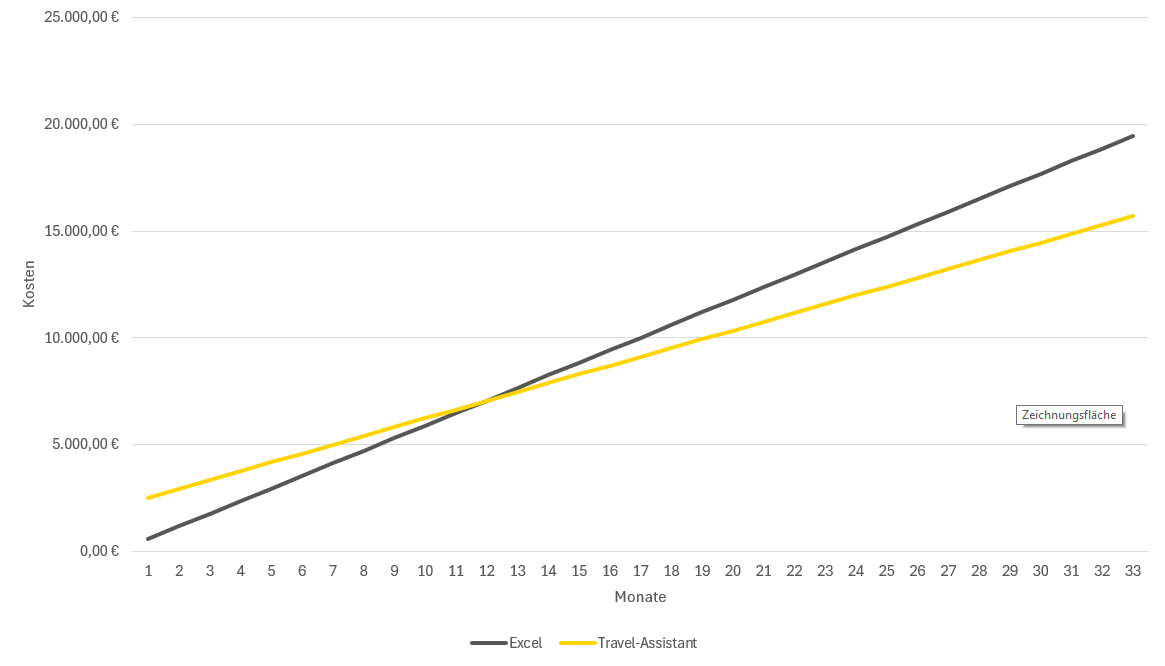
\includegraphics[width=1\textwidth]{amortisationsrechnung.png}

Damit ergibt sich ein Break Even Point bei ungefähr 12 Monaten.

Diese Annahmen basieren auf Durchschnitts- oder Erwartungswerten, von denen realistischerweise ausgegangen werden kann.
Detailierte Berechnung ist im Anhang unter \sct{sec:Anhang:Amortisationsrechnung}{Amortisationsrechnung} zu finden.

\subsection{Anwendungsfälle und Benutzerklassifizierung}
\label{sec:Analysephase:Benutzerklassifizierung}

Um herauszufinden, auf welche Art und Weise das Berechtigungskonzept aussehen sollte, wurde analysiert, welche Personengruppen wie mit der Softwarelösung arbeiten müssen.
Grundsätzlich lassen sich folgende drei Personengruppen feststellen:

\begin{enumerate}
    \item \emph{Reguläre Benutzer}\\
    Jede mitarbeitende Person, die berechtigt ist, \glp{RA} einzureichen.
    \item \emph{Vorgesetzte/\gl{GF}}\\
    Personen, die berechtigt sind, \glp{RA} anderer Personen zu bestätigen.
    \item \emph{Prüfer}\\
    Personen, die berechtigt sind, \glp{RA} auf ihre Richtigkeit zu prüfen.
\end{enumerate}

Im Anhang ist ein \sct{sec:Anhang:Anwendungsfalldiagramm}{Anwendungsfalldiagramm} zu finden welches, mögliche Aktionen der jeweiligen Personengruppen zuordnet.

\section{Planungsphase}
\label{sec:Planungsphase}
Nachdem die aktuelle Situation analysiert wurde, wurde mit der Planung der Applikation begonnen.

\subsection{Applikationsart}

Wie bereits unter \sct{sec:Einführung-Definitionsphase:Projektziel}{Projektziel} genannt, soll die Applikation als Webapplikation entwickelt werden. Ein Grund dafür ist, dass man die Applikation so in der Zukunft
vergleichsweise einfach aktualisieren kann. Der Technologie Stack \gl{MERN} wirf für die Erstellung der Softwarelösung gewählt, weil diese generell Etabliert und bereits in dem Software Development Team verwendet wird und in diverse Projekten bereits umgesetzt wird. Dadurch kann gegebenenfalls vom Know-How anderer Personen im Team profitiert werden. So wird die Serverapplikation mit \gl{express} auf der Laufzeitumgebung \gl{nodejs} entwickelt werden. Die \gl{SPA} mit \gl{React} entwickelt werden und \gl{MongoDB} zur Speicherung von Daten verwendet werden.

\subsection{Applikationsarchitektur}
\label{sec:Planungsphase:Applikationsarchitektur}

Die Softwarelösung wird in zwei Teilapplikationen entwickelt: \sct{sec:Planungsphase:Frontend}{Frontend} und \sct{sec:Planungsphase:Backend}{Backend}. Eine Backend Applikation ist Notwenig da sich bereits auf eine \gl{SPA} festgelegt wurde. Da eine \gl{SPA} nicht sicher mit Daten interagieren kann.

\subsubsection{Frontend}
\label{sec:Planungsphase:Frontend}

Das Frontend wird durch eine \gl{SPA} repräsentiert. Eine \gl{SPA} ist eine Applikation, die vollständig im Browser ausgeführt wird.  Im Gegensatz zu normalen Webanwendungen wird nicht bei jeder Interaktion mit dem Server \gl{HTML} zurückgegeben und vom Browser dargestellt.Stattdessen wird die Interaktion durch browserseitiges \gl{JS} ausgeführt.

\subsubsection{Backend}
\label{sec:Planungsphase:Backend}

Das Backend läuft auf dem Server und und übernimmt die gesamte Datenverwaltung und Businesslogik. Mit \gl{mongoose} kann das Backend dann auf die gespeicherten Daten der \gl{MongoDB} zugreifen.

Da die beiden Teilapplikationen miteinander kommunizieren müssen stellt das Backend eine \gl{HTTP}-\gl{API} zur Verfügung. Über diese kann dann das Frontend Informationen senden. Um so z.B. \glp{RA} einreichen zu können.
Das Backend wird auf Basis der \gl{MSC}-Architektur entwickelt. Dabei werden die Komponenten nach Typ unterteilt. In der \gl{MSC}-Architektur gibt es folgende Komponententypen:

\begin{enumerate}
  \item \textbf{M}odel\\
  Das Model beschreibt die zu speichernden Daten im Rahmen einer einzelnen Entität. So werden im Model die klassischen CRUD-Operationen durchgeführt. Wie das Kreieren einer \gl{RA}.
  \item \textbf{S}ervice\\
  Im Service findet die gesamte Logik statt. Services sind die einzigen Komponenten der Applikation, die mit Models interagieren. Sie bieten die Möglichkeit, die CRUD-, und gegebenenfalls noch weitere, Operationen auszuführen. Wie die Hintergrundberechnungen von Pauschalen.
  \item \textbf{C}ontroller\\
  Controller sind die Komponenten, die die tatsächliche Interaktion mit der Außenwelt, also dem \gl{HTTP}-Client bestreiten. Sie interagieren mit den Services, um die Anfragen des Clients auszuführen. Der Punkt, an dem die Daten vom Frontend an die Services zur Verarbeitung gesendet werden.
\end{enumerate}

Neben diesen Hauptkomponenten gibt es die folgenden Komponenten:

\begin{itemize}
  \item Middleware\\
Neben den vorinstallierten oder heruntergeladenen Middlewares können auch eigene erstellt werden. Im konkreten Fall wird eine Middleware verwendet, die den Zugriff auf bestimmte Bereiche der Applikation einschränkt. Dadurch wird eine Anfrage bereits vor dem Eintreffen im Controller beantwortet, falls bestimmte Anforderungen nicht erfüllt sind. So können z.B. nur Benutzer mit der Prüfer Rolle die Prüfungsansicht einsehen.
  \item Tests\\
  Die Tests dienen dazu, die einzelnen Komponenten auf verschiedene erwartete Ergebnisse hin zu überprüfen. Dabei werden die kritischen Berechnungsfunktionen auf ihr vorgesehenes Verhalten geprüft.
\end{itemize}

\subsection{Models und Datenstruktur}

Die Anforderungen machen deutlich, dass mehrere Modelle erforderlich sind. So wird ein Modell für die Länder und deren Pauschalen benötigt. Die Reisekostenabrechnung selbst, die sich aus dem Chatverlauf ergibt, sowie Grundinformationen und Dienstreisen welche die Informationen aus dem Chat verarbeitet. Sowie ein Modell, das einige Berechnungsgrundlagen speichert. Außerdem wird ein Benutzermodell benötigt, um die jeweiligen Vorgesetzten zu speichern.

\subsection{Feststellung der Benutzerberechtigungen}
\label{sec:Planungsphase:Benutzerberechtigungen}

Das unter \sct{sec:Analysephase:Benutzerklassifizierung}{Benutzerklassifizierung} beschriebene Benutzerkonzept sieht drei Benutzerklassen vor. Es wird davon ausgegangen, dass jeder Benutzer, der sich an der Anwendung bzw. am \gl{IDP} anmeldet, zunächst ein Regulärer Benutzer ist. Anschließend wird geprüft, ob ein Benutzer über eine Rolle verfügt, die ihm über den \gl{IDP} zugewiesen wurde.


\section{Durchführungsphase}
\label{sec:Durchführungsphase}
\input{sections/durchführungsphase}

\section{Abschlussphase}
\label{sec:Abschlussphase}
\subsection{Soll/Ist-Vergleich}
\label{sec:Abschlussphase:Soll/Ist-Vergleich}

Das Projekt wurde wie geplant umgesetzt. Allerdings konnte der Zeitplan nicht vollständig eingehalten werden:

In der Projektdefinitionsphase konnte die eingeplante Zeit eingehalten und sogar verkürzt werden. Die Ist-Analyse fiel aufgrund diverser in der Vergangenheit liegender Berührungspunkte relativ einfach aus.

Die Planungsphase des Projekts wurde grundsätzlich eingehalten, jedoch gab es kleinere Schwankungen, die innerhalb dieser Phase durch andere ausgeglichen wurden. Für das Erstellen des Anwendungsfalldiagramms und der Sketche musste weniger Zeit aufgewendet werden, da im schulischen Kontext eine Auffrischung stattfand. Aufgrund von Speicherproblemen während der Entwicklung musste die Datenbank mehrmals angepasst werden.

Die Projektdurchführungsphase nimmt den Großteil der Stunden in Anspruch. Diese Phase hat mehr Zeit benötigt als ursprünglich geplant. Für die Erstellung der Docker-Umgebung und der Grundstruktur der Webanwendung wurde weniger Zeit benötigt, da dies aufgrund der regelmäßigen Anwendung in anderen Projekten schneller umgesetzt werden konnte als ursprünglich geplant. Bei der Berechnungslogik konnte einiges an Zeit eingespart werden. Der Grund dafür liegt in wegfallenden Berechnungen/Feldern, die nicht mehr benötigt werden. Dadurch ist auch der Aufwand für die Tests dieser kritischen Funktionen geringer geworden. Der Aufwand für die Erstellung und Strukturierung der Fragen wurde jedoch unterschätzt. Um den Überblick über die Abfolge der Fragen zu behalten, musste ein Decision Tree erstellt werden (Im Anhang unter \sct{sec:Anhang:DecisionTree}{Decision Tree} zu finden), um nachvollziehen zu können, an welcher Stelle sich der Code/Chat befindet und zu welcher Abfolge von Fragen dieser führt. Bei der Implementierung der Mobil-First-Oberflächen hat die Verwendung des Frameworks \gl{React} anfangs Schwierigkeiten bereitet und zusätzliche Recherche erfordert. Auch die Integration des \gl{IDP} hat mehr Zeit in Anspruch genommen, da der Autor bisher nur Server-Side-Applikationen mit dem \gl{IDP} verbunden hat. 

In der Projektabschlussphase konnte wiederum Zeit gewonnen werden, da die Abnahme nur aus einer Präsentation des Tools und einem Ausblick bestand, da die Softwarelösung in der ersten Version noch nicht produktiv einsetzbar ist. Auch bei der internen Dokumentation wurde Zeit eingespart, da parallel zum Erstellen von Funktionen eine entsprechende Dokumentation mithilfe von \gl{JSdoc} erstellt wurde. Die Zeit für die Erstellung der Projekt-Dokumentation ist höher als geplant, aufgrund ihres Umfangs.

Eine Detailierter Vergleich zu den geplanten und tatsächlich benötigten Stunden für die jeweiligen Phasen und Arbeitspakete ist im Anhang unter \sct{sec:Anhang:sollistvergleich}{Soll-/Ist Zeitplan} zu finden.

\subsection{Lessons Learned}
\label{sec:Abschlussphase:Lessons Learned}

Im Laufe des Projekts gab es wie auch zuvor im \sct{sec:Abschlussphase:Soll/Ist-Vergleich}{Soll/Ist-Vergleich} beschrieben einige Herausforderungen. Welche jedoch überwunden werden konnten. Die Erstellung dieser Softwarelösung und die einhergehenden Lerneffekte haben sich als sehr Wertvoll erwiesen. So konnten Fähigkeiten im Bereich der Frontendentwicklung deutlich gefestigt und erweitert werden, da der Fokus im sonstigen Arbeitsaltag auf der Backendentwicklung liegt. Planung ist sehr wichtig, das hat sich in bei dem erstellen der Softwarelösung deutlich bemerkbar gemacht. Das Projekt verlief ohne große Hürden da in vielen Phasen auf die Planung der vorangegangen Phasen zurückgegriffen werden konnte.

\subsection{Ausblick}
\label{sec:Abschlussphase:Ausblick}
Wie bereits erwähnt, ist die Softwarelösung in seiner jetzigen Form noch nicht produktiv einsetzbar. Es werden noch einige Funktionalitäten benötigt:

\begin{itemize}
    \item Englische Übersetzung für nicht Deutschsprachige Kollegen
    \item Benachrichtigungen per E-Mail (z.B. Freigaben oder Status Änderungen)
    \item Konfiguration von Pauschalen
    \item Logging von Benutzer Aktionen
\end{itemize}


\section{Glossar}
\printnoidxglossary[title={Glossar}, type=main]

\section{Anhang}

\subsection{MicrosoftExcelDatei}
\label{sec:Anhang:MicrosoftExcelDatei}
\begin{landscape}
    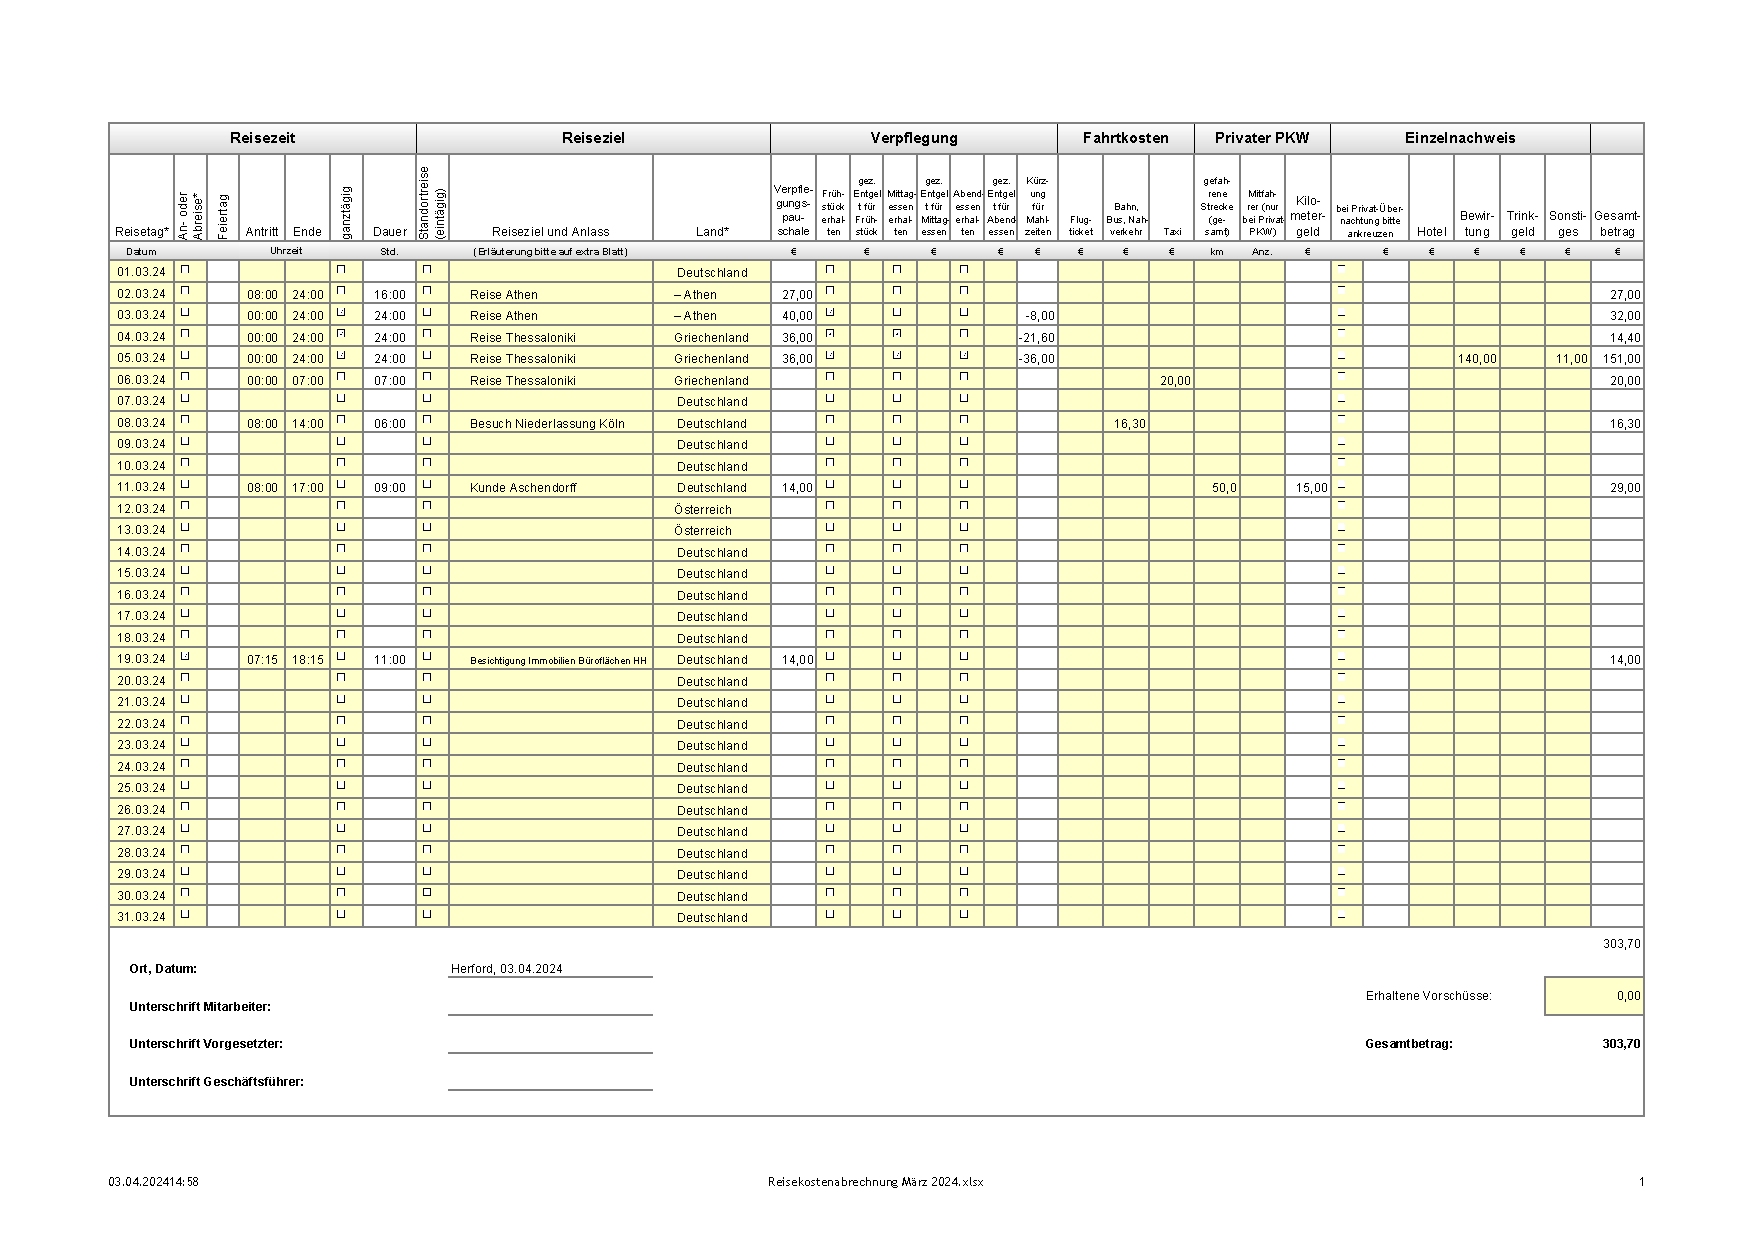
\includepdf[landscape=true]{microsoftexceldatei.pdf}
\end{landscape}
\pagebreak

\subsection{Lastenheft}
\label{sec:Anhang:Lastenheft}
\textbf{Zieldefinition}\\
Digitalisierung von Erstellung, Verwaltung \& Validierung der Reisekostenabrechnungen mithilfe einer Single-Page-Application (SPA).

\textbf{Ist Zustand}\\
Mitarbeiter im Außendienst müssen für Dienstreisen eine Reisekostenabrechnung (im Folgenden: RA) erstellen. Diese RA muss bis zum 8. des Folgemonats eingereicht werden. Bisher erstellten die Außendienstmitarbeiter die Reisekostenabrechnung mit Hilfe einer komplexen und sehr unübersichtlichen Microsoft-Excel-Dateivorlage (im Folgenden Excel-Datei genannt). Aufgrund dieser Komplexität und der fehlenden Hilfestellung kommt es vor allem bei den ersten Anwendungen zu vielen Rückfragen in der Accounting Abteilung oder bei anderen Kollegen. In die Excel-Datei, die auch Berechnungen durchführt, müssen verschiedene Angaben zur Dienstreise eingetragen werden. Nachdem die Excel-Datei ausgefüllt wurde, muss diese ausgedruckt und vom Vorgesetzten genehmigt und unterschrieben werden. Wurde die RA genehmigt, muss diese mit Quittungen bzw. Belegen per „Hauspost“ (interner Abhol- und Postdienst am Standort Herford), was im günstigsten Fall einen halben Tag dauert, oder per Post, was 2-3 Tage dauert, an die Buchhaltung geschickt werden.
Diese prüfen die RAs und geben sie bei Fehlern an den Außendienstmitarbeiter zur Anpassung zurück. Ist die RA korrekt ausgefüllt \& sind die notwendigen Belege \& Quittungen vorhanden, wird diese dann an die Payroll Accounting Abteilung weitergeleitet, damit die Reisekosten erstattet werden können.

\textbf{Soll Zustand}\\
Die Excel-Datei soll durch eine moderne SPA ersetzt werden. Diese SPA soll die Möglichkeit bieten, eine RA digital zu erstellen, freizugeben und zu prüfen. Die Außendienstmitarbeiter sollen mit Hilfe eines regelbasierten Chatbots durch das Ausfüllen einer RA geführt werden. Die Bearbeitung soll jederzeit zu einem anderen Zeitpunkt fortgesetzt werden können. Sobald alle notwendigen Angaben gemacht wurden, kann der Außendienstmitarbeiter die RA freigeben. Diese muss dann zunächst vom jeweiligen Teamleiter/Vorgesetzten über die SPA bestätigt werden, bevor sie der Accounting Abteilung zur Prüfung vorgelegt wird. Die SPA sollte dann die Berechnungen der RA aufschlüsseln, damit die Buchhaltung diese besser nachvollziehen/prüfen kann. Werden Unstimmigkeiten/Unvollständigkeiten festgestellt, so wird die RA mit dem entsprechenden Vermerk zur Bearbeitung an den Außendienstmitarbeiter zurückgegeben und nach Anpassung wieder an die Accounting Abteilung freigegeben. Sobald die RA fehlerfrei ist, kann die Accounting Abteilung eine Auszahlung veranlassen lassen.

\textbf{Funktionale Anforderungen}
\begin{enumerate}
	\item Datenbank + Anbindung zur Speicherung
	\begin{enumerate}
		\item Vollständige/ Unvollständige RA Daten speichern können
		\item RA Daten speichern können
		\item Belege (Bilder) speichern können
	\end{enumerate}
	\item Erstellung einer RA
	\begin{enumerate}
		\item Erstellung durch ein Regelbasierenden Chatbot
		\item Möglichkeit bieten zu gewissen „fragen“ zusätzlich belege hochzuladen
	\end{enumerate}
	\item Übersicht der RAs
	\begin{enumerate}
		\item Nutzer können alle selbst erstellten RAs einsehen
		\item Anzeige des jeweiligen Status der RAs
	\end{enumerate}
	\item Übersicht Freigabe der RAs
	\begin{enumerate}
		\item Vorgesetzte haben eine Übersicht über eingereichte RAs für ihre zuständigen Mitarbeiter
	\end{enumerate}
	\item Freigabe/Ablehnung von RAs durch Vorgesetzten
	\item Übersicht Prüfung der RAs
	\begin{enumerate}
		\item Prüfer können alle vom Nutzer \& Vorgesetzten Freigegebenen RAs einsehen
	\end{enumerate}
	\item Prüfung der RAs
	\begin{enumerate}
		\item Prüfer haben eine detaillierte Ansicht der RA
		\item Prüfer haben eine Aufschlüsselung der Berechnungen einer RA
		\item Prüfer haben die Möglichkeit Vermerke zu schreiben
		\item Prüfer haben die Möglichkeit die RA freizugeben oder zurückzusenden 
	\end{enumerate}
	\item Statische Implementierung von Pauschalen
	\begin{enumerate}
		\item Kilometer Pauschale
		\item Länder Pauschalen
		\begin{enumerate}
			\item Pauschalbeträge 8-24 Std. oder (An/Abreisetag)
			\item Pauschalbeträge Ganztags
			\item Pauschalbeträge Privatübernachtung
		\end{enumerate}
		\item Prozentuale Abzüge für erhaltene Mahlzeiten
	\end{enumerate}
	\item Berechnung von Pauschalen
	\begin{enumerate}
		\item Pauschalen/Werte sollen im Hintergrunde anhand der Benutzer Angaben berechnet werden
		\item Nachvollziehbarkeit soll für Prüfer gegeben sein
	\end{enumerate}
	\item Login, Rechte und Benutzer Verwaltung
	\begin{enumerate}
		\item Integration des Hauseigenen Identity Providers (IDP)
		\item Benutzer \& Rechte werden über den hauseigenen IDP verwaltet
	\end{enumerate}
\end{enumerate}

\textbf{Nicht Funktionale Anforderungen}
\begin{enumerate}
	\item Benutzung des Corporate Designs
	\item Sprache für die Oberflächen: Deutsch
	\item Erstellung von RAs soll durch Fragestellungen vom Regelbasierenden Chatbot auch für neu Einsteiger selbsterklärend sein
	\item Zwischen Speicherung 
	\begin{enumerate}
		\item Von RAs
		\item Von Prüfungen der RAs
	\end{enumerate}
	\item Intuitive Benutzung
\end{enumerate}

\textbf{Rollen}
\begin{itemize}
	\item Regulärer Benutzer – Mitarbeiter im Außendienst
	\item Prüfer – Mitarbeiter in der Accounting Abteilung
	\item Vorgesetzter - Übergeordneter Mitarbeiter des Außendienst Mitarbeiters
\end{itemize}

\textbf{Status}
\begin{itemize}
	\item Offen – noch nicht zur Prüfung/Freigabe gesendete RA
	\item In Bearbeitung – RA ist zur Bearbeitung/Freigabe bei der Accounting Abteilung/ Vorgesetzten
	\item Fehlerhaft – RA wurde mit einem Vermerk zurück gegeben
	\item Fertig – Wurde erfolgreich abgearbeitet
\end{itemize}

\textbf{Abnahme- und Testkriterien}
\begin{enumerate}
	\item Reibungslose Erstellung und Verwaltung von RAs sowie die Prüfung soll gegeben sein
	\item Erfüllt alle Funktionalen Anforderungen
	\item Ist auf Server Lauffähig
	\item Code abschnitte, welche Berechnungen anhand von Pauschelen durchführen müssen ausführlich getestet und auf Richtigkeit geprüft werden
\end{enumerate}

\pagebreak

\subsection{Verwendete Ressourcen}
\label{sec:Anhang:VerwendeteRessourcen}

\begin{enumerate}
    \item Hardware \\
    \begin{itemize}
        \item Betrieblich bereitgestellter Bildschirmarbeitsplatz (2x Monitor, Tastatur, Maus, Dockingstation)
        \item Betrieblich bereitgestelltes Notebook
    \end{itemize}
    \item Software \\
    \begin{itemize}
        \item Windows 11
        \item Visual Studio Code
        \item Git
        \item Docker
        \item Node.js
        \item Windows Terminal
        \item Firefox Developer Edition
        \item Draw.io
        \item TeXworks
        \item Texmaker
    \end{itemize}
\end{enumerate}

\pagebreak

\subsection{Soll-/Ist-Zeitplanung}
\label{sec:Anhang:sollistvergleich}
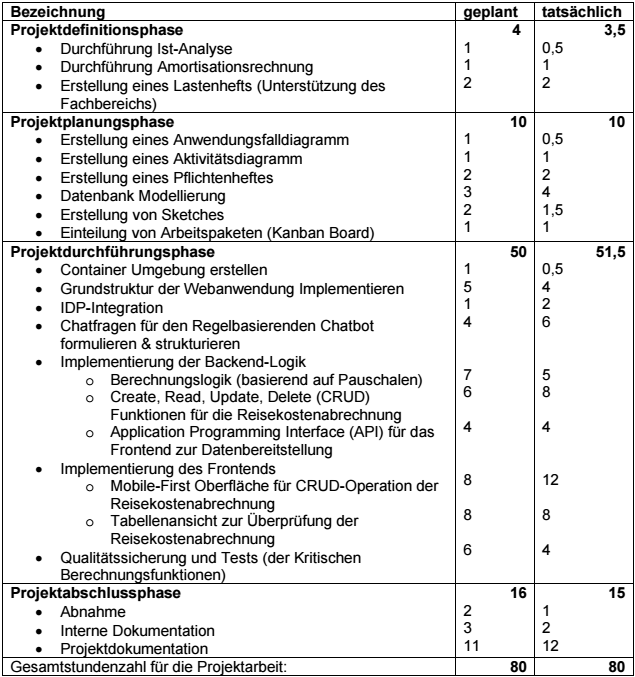
\includegraphics[width=1\textwidth]{sollistvergleich.png}
\pagebreak

\subsection{Prozess Alt}
\label{sec:Anhang:ProzessAlt}
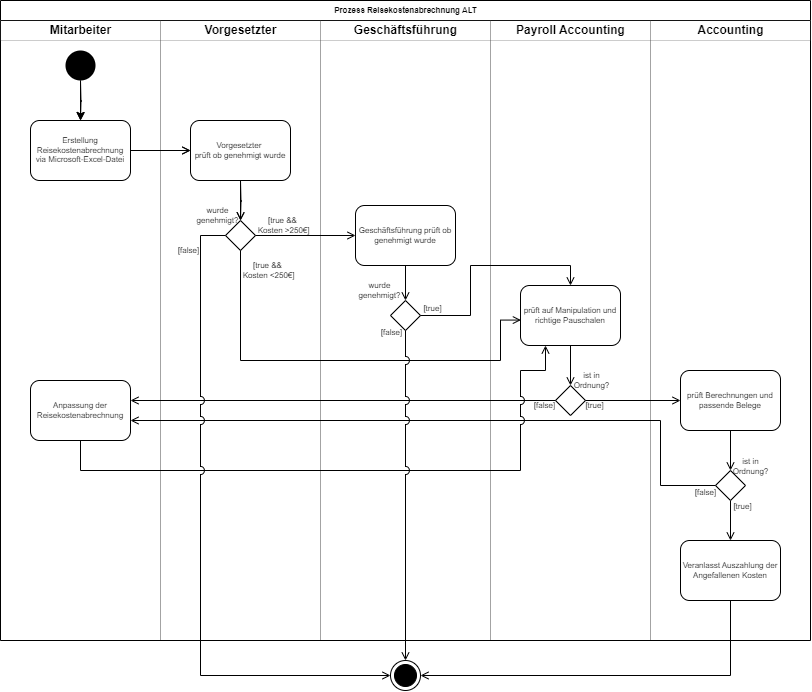
\includegraphics[width=1\textwidth]{prozessreisekostenabrechnungalt.png}
\pagebreak

\subsection{Amortisationsrechnung}
\label{sec:Anhang:Amortisationsrechnung}

Berechnung der monatlichen Kosten durch die aktuelle Lösung:\\
	\glp{RA} erstellen: \[ 20 \glp{RA} \cdot \displaystyle\frac{15minuten}{60minuten} \cdot 25€/h =  \bf{125,00€} \]
	Einarbeitung \gl{MA} im Außendienst: \[ 0,5 \cdot 2 \gl{MA} \cdot 25€/h =  \bf{25,00€} \]
	Aushelfen: \[ 20\% \cdot 20 \glp{RA} \cdot 2 \gl{MA} \cdot \displaystyle\frac{15minuten}{60minuten} \cdot 25€/h = \bf{50,00€} \]
	Genehmigung Vorgesetzter:  \[ 20 \glp{RA} \cdot \displaystyle\frac{5minuten}{60minuten} \cdot 45€/h =  \bf{75,00€} \]
	Genehmigung \gl{GF}:  \[ 1 \glp{RA} \cdot \displaystyle\frac{5minuten}{60minuten} \cdot 100€/h =  \bf{8,33€} \]
	Hauspost:  \[ 90\% \cdot 20 \glp{RA} \cdot \displaystyle\frac{10minuten}{60minuten} \cdot 7€/h =  \bf{21,00€} \]
	Selbst gebracht:  \[ 10\% \cdot 20 \glp{RA} \cdot \displaystyle\frac{10minuten}{60minuten} \cdot 25€/h =  \bf{8,33€} \]
	Prüfung Payroll Accounting: \[ 20 \glp{RA} \cdot \displaystyle\frac{10minuten}{60minuten} \cdot 30€/h =  \bf{100,00€} \]
	Prüfung Accounting: \[ 20 \glp{RA} \cdot \displaystyle\frac{12minuten}{60minuten} \cdot 30€/h =  \bf{120,00€} \]
	Nachbearbeitung: \[ 25\% \cdot 20 \glp{RA} \cdot \displaystyle\frac{10minuten}{60minuten} \cdot 25€/h =  \bf{20,83€} \]
	Nachprüfung: \[ 25\% \cdot 20 \glp{RA} \cdot \displaystyle\frac{7minuten}{60minuten} \cdot 30€/h =  \bf{17,50€} \]
	Rückfragen Accounting: \[ 10\% \cdot 20 \glp{RA} \cdot \displaystyle\frac{10minuten}{60minuten} \cdot (25€/h + 30€/h) =  \bf{18,33€} \]

Summe der monatlichen Kosten durch die aktuelle Lösung:\\
\begin{multline}
  125€ + 25€ + 50€ + 75€ + 8,33€ + 21€ + 8,33€ + 100€ + 120€ + 20,83€ + 17,50€ + 18,33€ \\ = \bf{589,33€}
\end{multline}

Berechnung der monatlichen Kosten durch die neuentwickelte Softwarelösung:
	\glp{RA} erstellen: \[ 20 \glp{RA} \cdot \displaystyle\frac{20minuten}{60minuten} \cdot 25€/h =  \bf{166,67€} \]
	Aushelfen: \[ 10\% \cdot 20 \glp{RA} \cdot 2 \gl{MA} \cdot \displaystyle\frac{5minuten}{60minuten} \cdot 25€/h = \bf{50,00€} \]
	Genehmigung Vorgesetzter:  \[ 20 \glp{RA} \cdot \displaystyle\frac{5minuten}{60minuten} \cdot 45€/h =  \bf{75,00€} \]
	Genehmigung \gl{GF}:  \[ 1 \glp{RA} \cdot \displaystyle\frac{5minuten}{60minuten} \cdot 100€/h =  \bf{8,33€} \]
	Prüfung Accounting: \[ 20 \glp{RA} \cdot \displaystyle\frac{7minuten}{60minuten} \cdot 30€/h =  \bf{70,00€} \]
	Nachbearbeitung: \[ 10\% \cdot 20 \glp{RA} \cdot \displaystyle\frac{7minuten}{60minuten} \cdot 25€/h =  \bf{5,83€} \]
	Nachprüfung: \[ 10\% \cdot 20 \glp{RA} \cdot \displaystyle\frac{5minuten}{60minuten} \cdot 30€/h =  \bf{5,00€} \]
	Rückfragen Accounting: \[ 10\% \cdot 20 \glp{RA} \cdot \displaystyle\frac{10minuten}{60minuten} \cdot (25€/h + 30€/h) =  \bf{18,33€} \]
	Wartung: \[ 2 Std. \cdot 27€/h =  \bf{54,00€} \]
	
Summe der monatlichen Kosten durch die neuentwickelte Softwarelösung: \[166,67€ + 50€ + 75€ + 8,33€ + 70€ + 5,83€ + 5€ + 18,33€ +54€ =  \bf{411,50€} \]

Berechnung Entwicklungskosten des Travel-Assistant:
	Implementierung: \[ 80 Stunden \cdot 7€/h =  \bf{560,00€} \]
	Hilfestellung/Rat: \[ 5 Stunden \cdot 30€/h =  \bf{150,00€} \]
	Meetings: \[ 6 Stunden \cdot 2 \cdot 30€/h =  \bf{360,00€} \]
	Feedback/Testing: \[ 1 Stunden \cdot 25€/h =  \bf{25,00€} \]
Summe Projekt Entwicklungskosten: \[560€ + 150€ + 360€ + 25€ =  \bf{1.095,00€} \]

Berechnung Weiteretwicklungskosten:
	Weiterentwicklung: \[ 25 Stunden \cdot 27€/h =  \bf{675,00€} \]
	Zusätzliche Meetings: \[ 4 Stunden \cdot ( 27€/h + ( 2 \cdot 30€/h)€ =  \bf{348,00€} \]
Summe Weiteretwicklungsskosten: \[675€ + 348€ =  \bf{1.023,00€} \]

Summe Entwicklungskosten bis zum vollumfänglichen Einsatz: \[1.095€ + 1.023€ =  \bf{2.118,00€} \]

Berechnung des Break-even-Points: \[ \displaystyle\frac{2.118€}{589,33€ - 411,50€} \approx  \bf{11,91} \Rightarrow 12 \] 

Monatliche Kosteneinsparungen:
\[ 589,33€ - 411,50€ =  \bf{177,83€} \]

Nach etwa 12 Monaten haben sich die Entwicklungskosten durch die eingesparten Kosten amortisiert. Ab diesem Zeitpunkt spart die neu entwickelte Softwarelösung 177,83€ pro Monat.
\pagebreak

%\subsection{Pflichtenheft}
\label{sec:Anhang:Pflichtenheft}
\textit{Version 1.1}\\

\todo Das Pflichtenheft muss noch erstellt werden
\textbf{Projektbeschreibung}\\
\todo 
Das Projekt soll die erste Version einer Softwarelösung sein, welche in Zukunft die Aktuelle Methode der Erstellung von Reisekostenabrechnungen welche mit einer Microsoft Excel Datei erstellt wird, ablösen.  Hierzu wird dem Auftragsnehmer ein Zeitraum von 80 Stunden eingeräumt. 

\textbf{Anforderungen}\\
Die Funktionalen und Nicht-Funktionalen Anforderungen, welche im Lastenheft niedergeschrieben sind werden unverändert übernommen.

\textbf{Architektur}\\
Die Softwarelösung wird mit dem Technologie-Stack MERN entwickelt.
Somit wird die Softwarelösung in zwei Abschnitte unterteilt. Frontend welches React nutzt und Backend welches express auf einem Node.js Server nutzt. Die Daten werden in einer MongoDB gespeichert.
Die Jeweiligen Komponenten laufen Seperat in Docker Containern.
Programmiert wird die Softwarelösung in JavaScript geschrieben.

\textbf{Benutzeroberfläche}
Die Oberfläche wird für bestimmte Bereiche wie folgt umgesetzt:
Mobile-First:
- erstellen und bearbeiten von \glp{RA}
Desktop Ansicht:
- prüfen
- validieren
Ein grobes Layout der Oberflächen sind unter \sct{sec:Anhang:Sketches}{Sketches} zu finden.

Prozess

Zielsetzung
Eine Softwarelösung erstellen welche das Erstellen, Verwalten \& Validieren der Reisekostenabrechnungen mithilfe einer Single-Page-Application (SPA) Digitalisiert.
Anforderungen
Die Anforderungen werden wie im Lastenheft beschrieben vollumfänglich übernommen
Benutzerrollen und -berechtigungen
Die Benutzerrollen werden wie im Lastenheft beschrieben übernommen und erweitert:
•	Nutzer – Mitarbeiter im Außendienst
•	Prüfer – Mitarbeiter der Accounting Abteilung
•	GF – Geschäftsführung
•	Vorgesetzter - Übergeordneter Mitarbeiter des Außendienst Mitarbeiters

\textbf{Status}
Die Möglichen Stati einer RA werden aus dem Lastenheft übernommen und wie folgt ergänzt:
\begin{itemize}
\item \verb|pending|
\end{itemize}
'pending', 'verified', 'accepted', 'declined', 'needsEditing'

\textbf{Abnahme}
Eine Gewöhnliche Projektabnahme gibt es nicht. Da diese erste Version der Softwarelösung noch nicht Vollumfänglich eingesetzt werden kann, ist eine Präsentation dieser an den Kunden ausreichend. Hierfür sollen alle Funktionen 
  

%\pagebreak

\subsection{Anwendungsfalldiagramm}
\label{sec:Anhang:Anwendungsfalldiagramm}
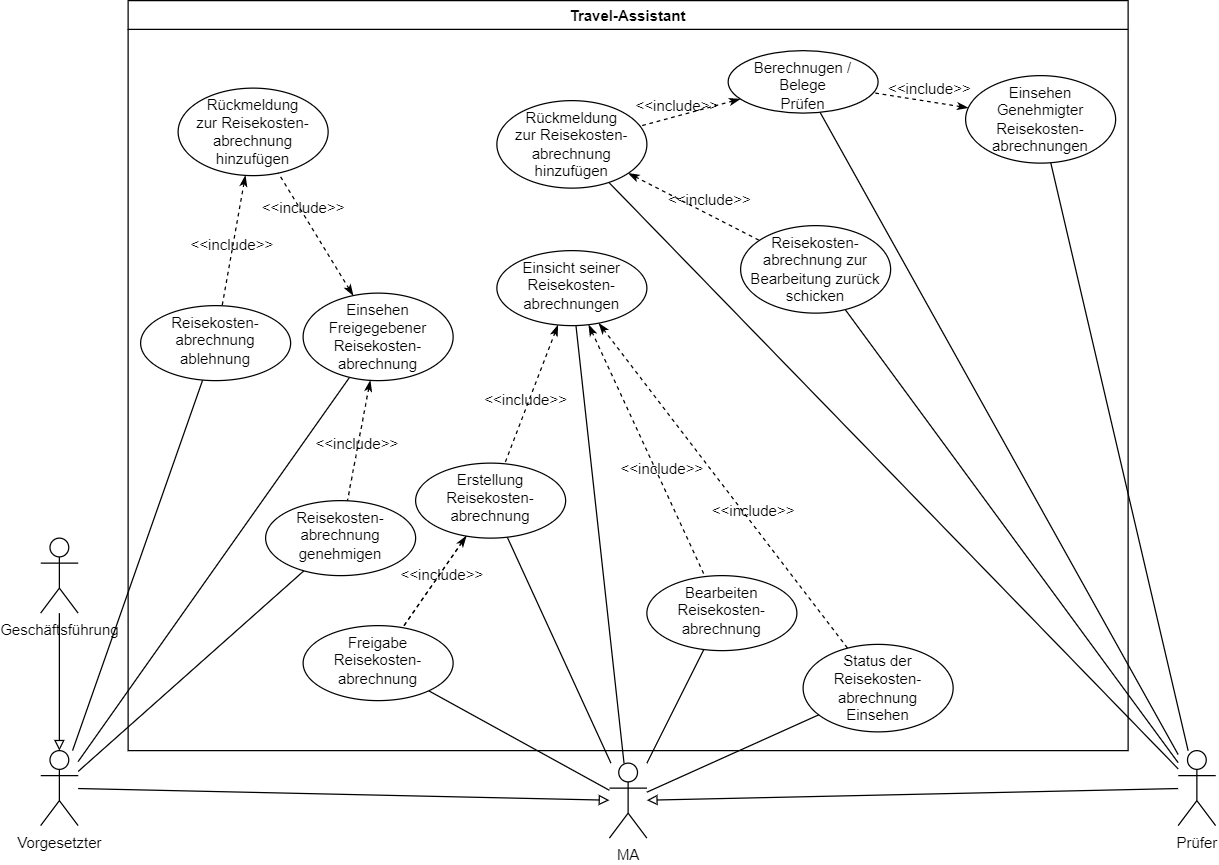
\includegraphics[width=1\textwidth]{anwendungsfalldiagramm.png}
\pagebreak

\subsection{IdP-Login}
\label{sec:Anhang:IdP-Login}
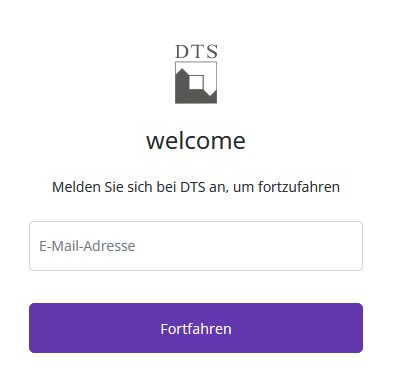
\includegraphics[width=0.5\textwidth]{emaillogin.png}

\includegraphics[width=0.5\textwidth]{pwlogin.png}
\pagebreak

\subsection{Kanban-Board}
\label{sec:Anhang:KanbanBoard}
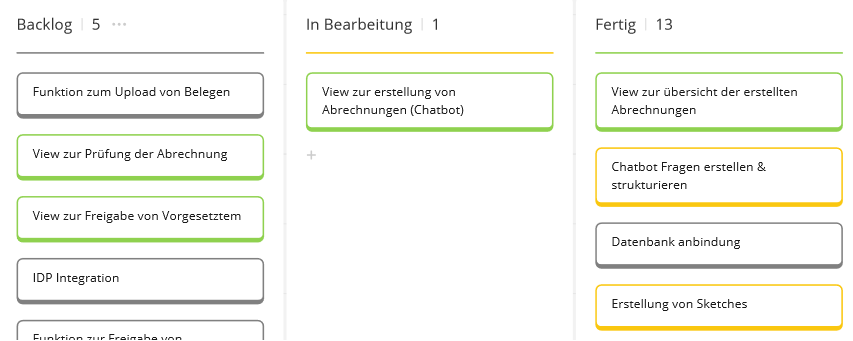
\includegraphics[width=1\textwidth]{kanbanboard.png}
\pagebreak

\subsection{Libraries}
\label{sec:Anhang:Libraries}

\subsubsection{Libraries (Backend)}
\label{sec:Anhang:Libraries:Backend}

\begin{table}[h]
    \centering
    \begin{tabular}{| l | l |}
        \hline
        \multicolumn{2}{|c|}{\textbf{dependencies}}\\
        \hline
        \textbf{Library} & \textbf{Kurzbeschreibung}  \\
        \hline
        axios & \gl{promise}-basierte \gl{HTTP}-Client-Library \\
        cookie-parser & Middleware für \gl{express}, um \gl{cookie}s zu lesen \\
        express & Middleware-basierte \gl{HTTP}-Server-Library \\
        mongoose & \gl{ODM} für \gl{MongoDB} \\
        dts-node-logger & Eine DTS Interner Logger für Node Applikationen \\
        dts-node-oidc-client & Eine DTS Interne Node OIDC Client Library \\
        eslint \& addons & Linter und Codeformatter \\
		jest & Testing Framework \\
		nodemon & Llibrary für automatischen Neustart bei Änderungen\\
		express-session & Library zum erstellen von Session-Middlewares\\
		connect-mongodb-session & Library zum speichern von Session Daten\\
		passport & Authentifizierungs-Middleware für \gl{nodejs}\\
		dotenv & Library zum Laden von Umgebungsvariablen \\
        \hline
    \end{tabular}
    \label{tab:libs-backend}
\end{table}

\subsubsection{Libraries (Frontend)}
\label{sec:Anhang:Libraries:Frontend}

\begin{table}[h]
    \centering
    \begin{tabular}{| l | l |}
        \hline
        \multicolumn{2}{|c|}{\textbf{dependencies}}\\
        \hline
        \textbf{Library} & \textbf{Kurzbeschreibung}  \\
        \hline
        axios & \gl{promise}-basierte \gl{HTTP}-Client-Library \\
        bootstrap & \gl{css}-Framework \\
        bootstrap-icons & Iconset von dem gleichen Team wie \verb|bootstrap| \\
        react & siehe \gl{React} \\
        react-bootstrap & \gl{React}-Components für \verb|bootstrap| \\
        react-bootstrap-icons & \gl{React}-Components für \verb|bootstrap-icons| \\
        react-dom & \gl{React}-Addon für den Browser \\
        react-router-dom & Routing-Funktionalität für \gl{React}-Applikationen im Browser \\
        react-multi-date-picker & \gl{React} datepicker component \\
        eslint \& addons & Linter und Codeformatter \\
        vite & siehe \gl{vite} \\
        \hline
    \end{tabular}
    \label{tab:libs-frontend}
\end{table}
\pagebreak

\subsection{Code-Ausschnitte}

\subsubsection{Berechnungs-Ausschnitt}
\label{sec:Anhang:Berechnungs-Ausschnitt}

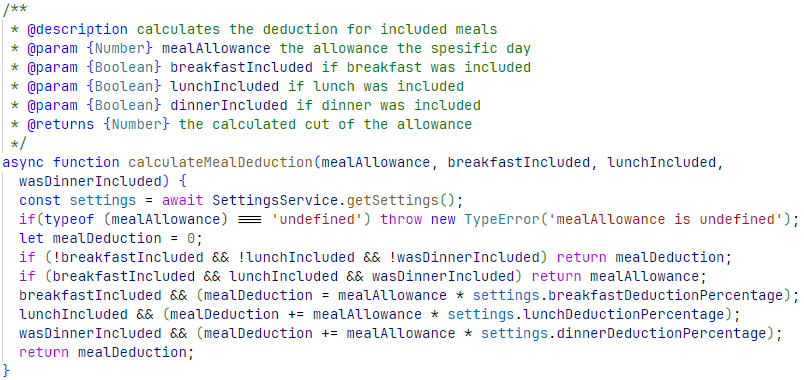
\includegraphics[width=1\textwidth]{codeausschnitt.png}

\subsubsection{Unittest-Ausschnitt}
\label{sec:Anhang:Unittest-Ausschnitt}

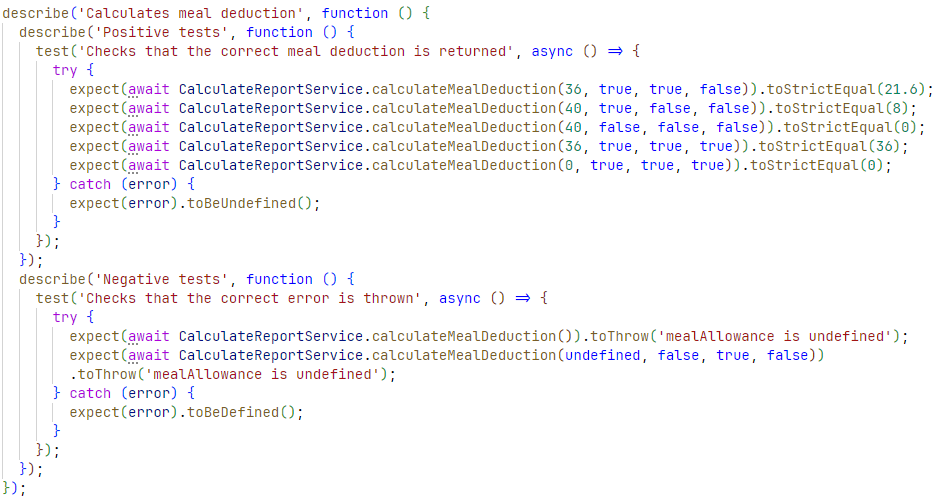
\includegraphics[width=1\textwidth]{unittestausschnitt.png}

\subsubsection{Chatbot-Ausschnitt}
\label{sec:Anhang:Chatbot-Ausschnitt}

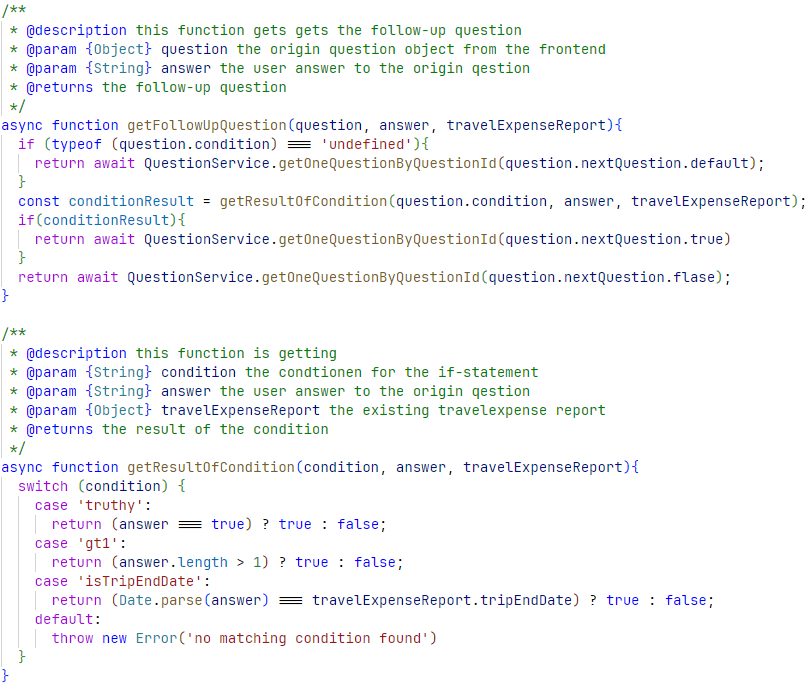
\includegraphics[width=1\textwidth]{chatbotlogik.png}

\subsection{Decision Tree}
\label{sec:Anhang:DecisionTree}
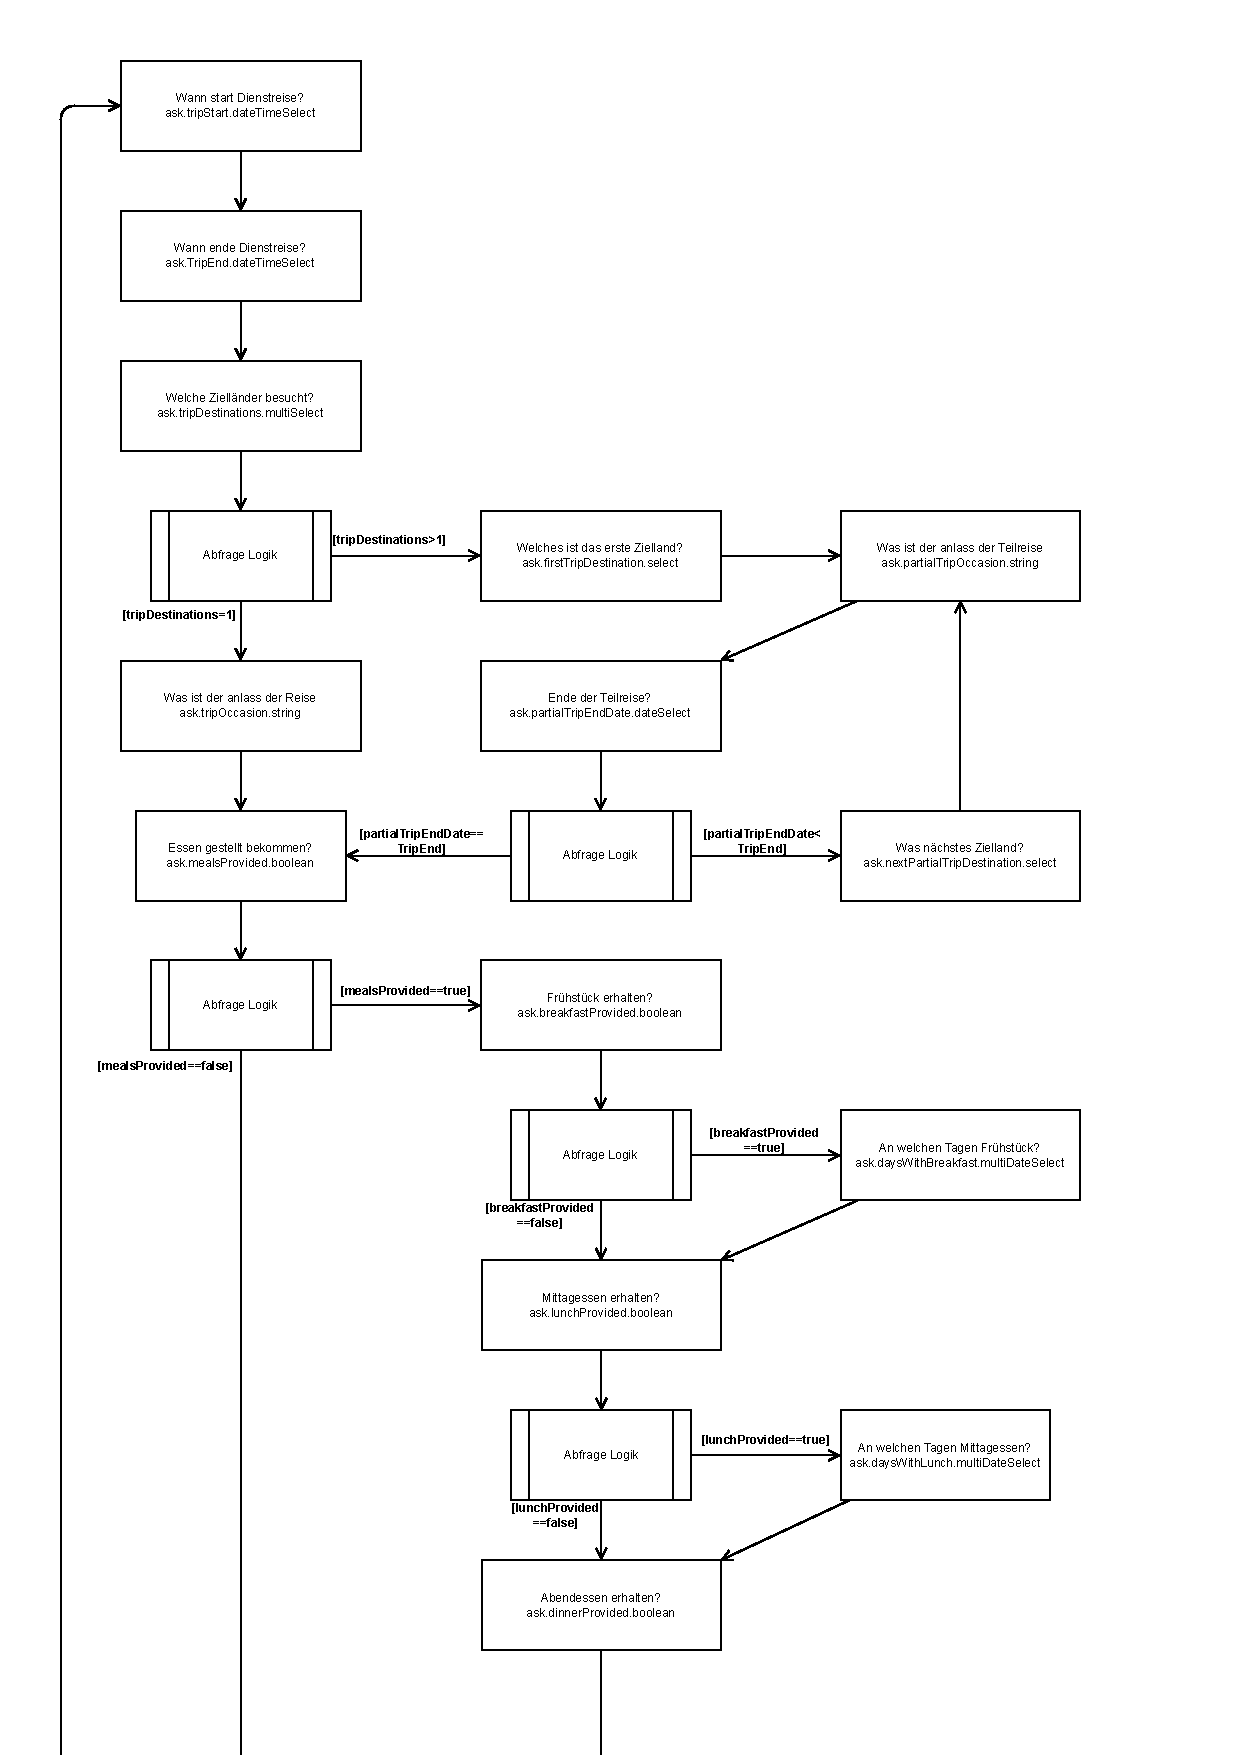
\includepdf[page=1-5]{decisiontree.pdf}

\subsection{Sketches}
\label{sec:Anhang:Sketches}

\begin{tabular}[h]{c|c|c}
\gl{RA} Übersicht & Chat & Chat bearbeiten
\includegraphics{sketchübersicht.png}& 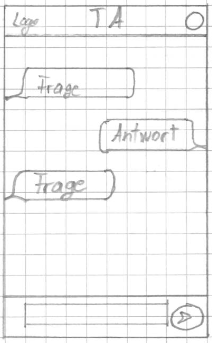
\includegraphics{sketchchat.png} & 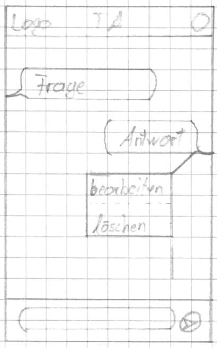
\includegraphics{sketchbearbeiten.png}
\hline
Beleg hochladen & Beleg gesendet & \gl{RA} freigeben
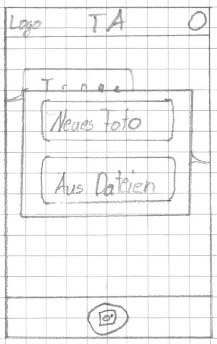
\includegraphics{sketchhochladen.png} & 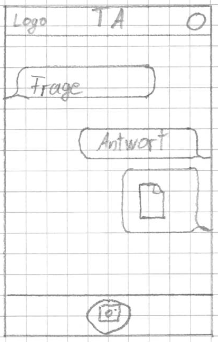
\includegraphics{sketchdatei.png}& 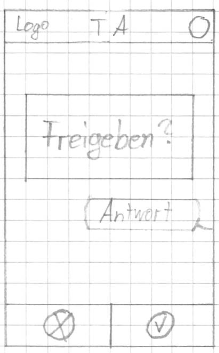
\includegraphics{sketchfreigeben.png}
\hline
\multicolumn{3}{c}{Prüfer Kommentar}}
\multicolumn{3}{c}{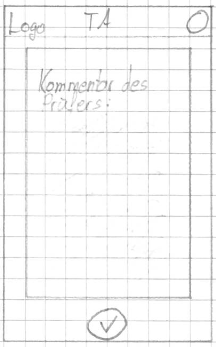
\includegraphics{sketchkommentar.png}}
\hline
\multicolumn{3}{c}{Prüfer übersicht der \glp{RA}}
\multicolumn{3}{c}{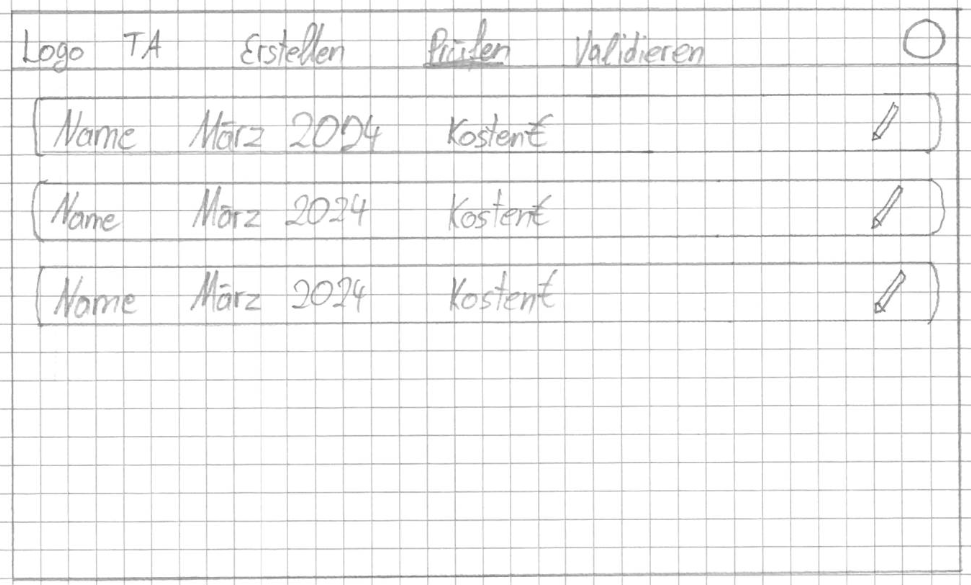
\includegraphics{sketchprüfungsübersicht.png}}
\hline
\multicolumn{3}{c}{Prüfungs ansicht einer \gl{RA}
\multicolumn{3}{c}{\includegraphics{sketchprüfung.png}}
\end{tabular}


\end{document}